% Copyright 2004 by Till Tantau <tantau@users.sourceforge.net>.
%
% In principle, this file can be redistributed and/or modified under
% the terms of the GNU Public License, version 2.
%
% However, this file is supposed to be a template to be modified
% for your own needs. For this reason, if you use this file as a
% template and not specifically distribute it as part of a another
% package/program, I grant the extra permission to freely copy and
% modify this file as you see fit and even to delete this copyright
% notice. 

\documentclass{beamer}

% There are many different themes available for Beamer. A comprehensive
% list with examples is given here:
% http://deic.uab.es/~iblanes/beamer_gallery/index_by_theme.html
% You can uncomment the themes below if you would like to use a different
% one:
%\usetheme{AnnArbor}
%\usetheme{Antibes}
%\usetheme{Bergen}
%\usetheme{Berkeley}
%\usetheme{Berlin}
%\usetheme{Boadilla}
%\usetheme{boxes}
%\usetheme{CambridgeUS}
%\usetheme{Copenhagen}
%\usetheme{Darmstadt}
%\usetheme{default}
%\usetheme{Frankfurt}
%\usetheme{Goettingen}
%\usetheme{Hannover}
%\usetheme{Ilmenau}
%\usetheme{JuanLesPins}
%\usetheme{Luebeck}
\usetheme{Madrid}
%\usetheme{Malmoe}
%\usetheme{Marburg}
%\usetheme{Montpellier}
%\usetheme{PaloAlto}
%\usetheme{Pittsburgh}
%\usetheme{Rochester}
%\usetheme{Singapore}
%\usetheme{Szeged}
%\usetheme{Warsaw}

\usepackage{media9}
\usepackage{textpos}

%\setbeamerfont{footline}{size=\fontsize{9}{11}\selectfont}

\title [Volcano Plume Modelling with SPH]{Data Management and Volcano Plume Simulation with
Parallel SPH Method and Dynamic Halo Domains}

% A subtitle is optional and this may be deleted
%\subtitle{Optional Subtitle}

\author [Zhixuan Cao ect.] {
    Zhixuan Cao\inst{1} \and
    Abani Patra\inst{1,3}  \and
    Matthew Jones\inst{2}
    }
% - Give the names in the same order as the appear in the paper.
% - Use the \inst{?} command only if the authors have different
%   affiliation.
%\institute[Universities of Somewhere and Elsewhere] % (optional, but mostly needed)
%{
%  \inst{1}%
%  Department of Computer Science\\
%  University of Somewhere
%  \and
%  \inst{2}%
%  Department of Theoretical Philosophy\\
%  University of Elsewhere}
  
\institute [University at Buffalo]{
\inst{1}
Department of Mechanical and Aerospace \\
University at Buffalo, Buffalo, New York, U.S.A.
\and
\inst{2}
Center for Computational Research \\
University at Buffalo, Buffalo, New York, U.S.A.
\and
\inst{3}
Computational, Data Sciences \& Eng.,\\
University at Buffalo, Buffalo, New York, U.S.A.
 }
% - Use the \inst command only if there are several affiliations.
% - Keep it simple, no one is interested in your street address.

\date [IHPCES 2017] {7th International Workshop on Advances in High-Performance Computational Earth Sciences: Applications $\&$ Frameworks, 2017}
% - Either use conference name or its abbreviation.
% - Not really informative to the audience, more for people (including
%   yourself) who are reading the slides online

\subject{Numerical modelling}
% This is only inserted into the PDF information catalog. Can be left
% out. 

% If you have a file called "university-logo-filename.xxx", where xxx
% is a graphic format that can be processed by latex or pdflatex,
% resp., then you can add a logo as follows:

%\pgfdeclareimage[height=0.5cm]{university-logo}{UB_Stacked_SUNY} \logo{\pgfuseimage{university-logo}}

% Delete this, if you do not want the table of contents to pop up at
% the beginning of each subsection:
\AtBeginSection[]
{
  \begin{frame}<beamer>{Outline}
    \tableofcontents[currentsection]
  \end{frame}
}

% Let's get started
\begin{document}

\begin{frame}
  \titlepage
\end{frame}

\addtobeamertemplate{frametitle}{}{%
\begin{textblock*}{350mm}(.80\textwidth,-0.85cm)

\includegraphics[height=0.75cm,width=2.5cm]{UB_Secondary_SUNY_Small}
\end{textblock*}}


\begin{frame}{Outline}
  \tableofcontents
  % You might wish to add the option [pausesections]
\end{frame}
%-----------------------------------------------------
% Section and subsections will appear in the presentation overview
% and table of contents.
\section{Motivation for Choosing SPH}
\begin{frame}{Motivation for Choosing SPH}
 Volcanic plume development is essentially a multi-phase, turbulent mixing process coupled with heat transfer and other microphysics processes without pre-defined boundaries. SPH (Smoothed particle hydrodynamics), as a mesh-less method, is suitable for such problems for several reasons:
  \begin{itemize}
  \item {
    SPH is able to automatically construct the interface.
  }
  \item {
    Multiphase modeling is easily accomplished using SPH 
  }
  \item {
    Adding of new physics and new phases is easier in terms of programming in SPH 
  }
  \item {
    With very limited global communication requirements, SPH solvers can scale better for parallel computing than grid based ones.
  }
  \end{itemize}
\end{frame}

\section{Overview}
\begin{frame}{Requirements of the application}
\begin{figure}[!t]
\centering
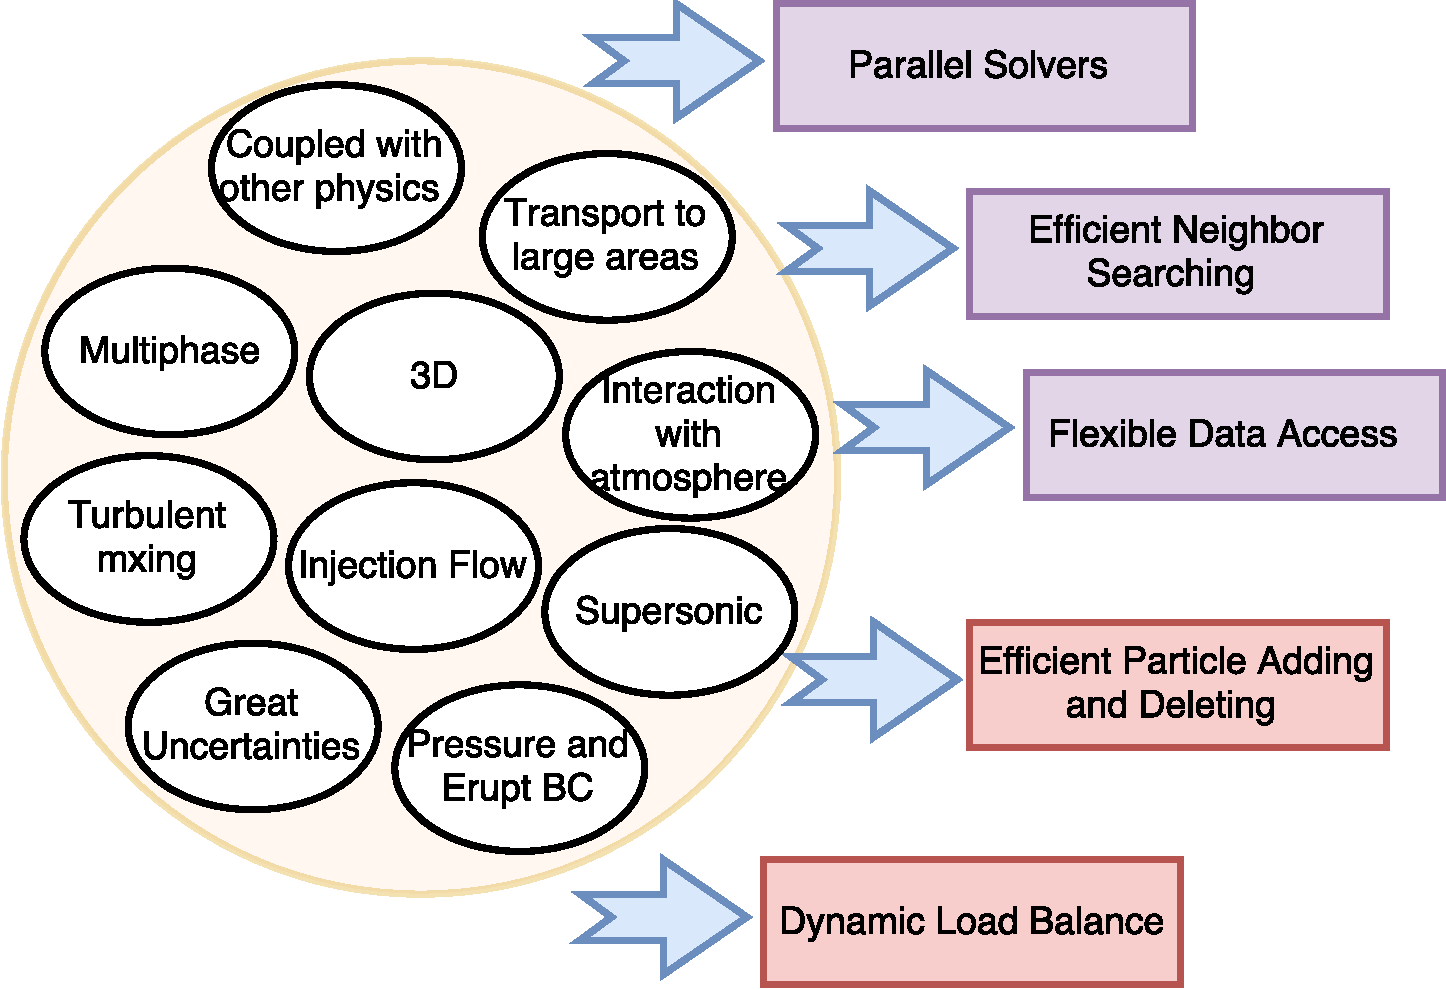
\includegraphics[scale=0.43]{Requirement}
%\caption{Scope of the problem}
\label{fig:Requirements}
\end{figure}
\end{frame}

\begin{frame}{Our Strategies}
\begin{figure}
\flushleft
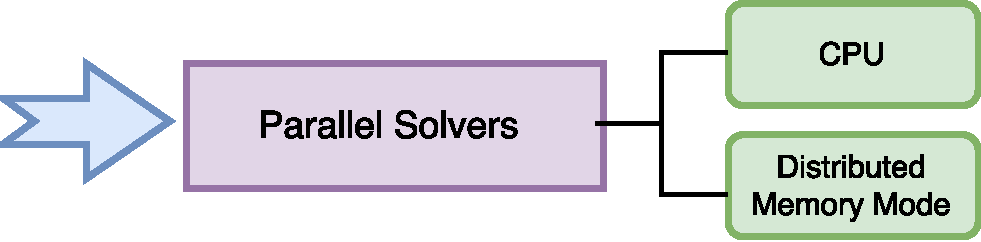
\includegraphics[scale=0.5]{Parallel}
%\caption{Scope of the problem}
\label{fig:Parallel}
\end{figure}
%
\begin{figure}
\flushleft

\includegraphics[scale=0.5]{NB_Search}
%\caption{Scope of the problem}
\label{fig:NB_Search}
\end{figure}
%
\begin{figure}
\flushleft
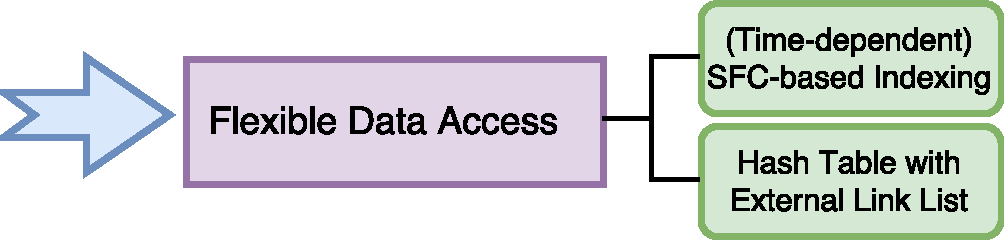
\includegraphics[scale=0.5]{Data_acc}
%\caption{Scope of the problem}
\label{fig:Data_acc}
\end{figure}
\end{frame}

\begin{frame}{Our Strategies}
\begin{figure}
\flushleft
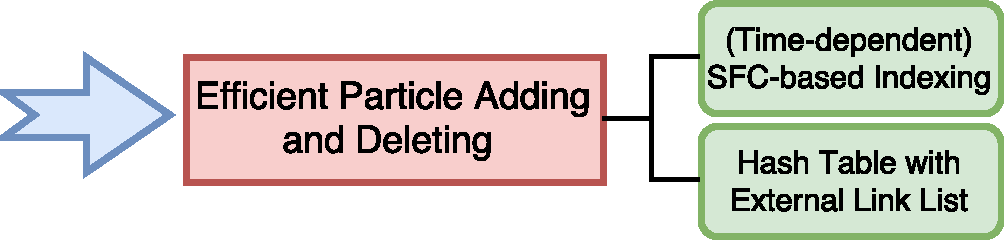
\includegraphics[scale=0.5]{P_add_del}
%\caption{Scope of the problem}
\label{fig:P_add_del}
\end{figure}
%
\begin{figure}
\flushleft
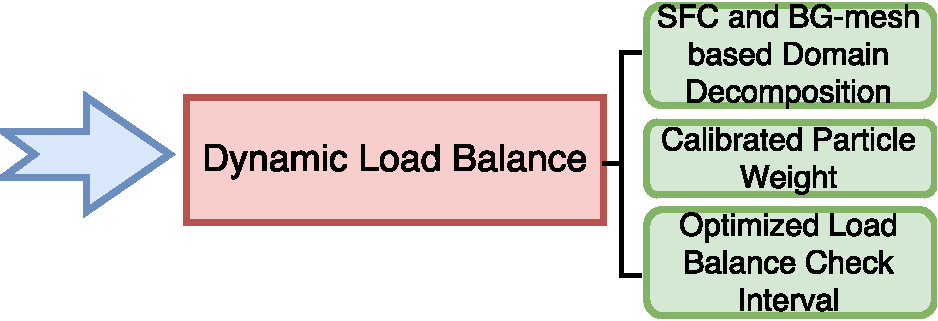
\includegraphics[scale=0.5]{Load_balance}
%\caption{Scope of the problem}
\label{fig:Requirements}
\end{figure}
\end{frame}

%-----------------------------------------------------
\section{Data Structure and Load Balance}
\begin{frame}{Paricles and Bucket}
The  basic data structures used to support SPH are particles and buckets. %Both are need as $C++$ classes.
\begin{block}{Particle Class}
Information that is contained in particle objects :
Unique ID (key), affiliation, {\bf primary variables, secondary variables}, flags and neighbor information.
\end{block}
\begin{block}{Bucket Class}
Information that is contained in bucket objects :
Unique ID (key), affiliation, dimension information, flags, neighbor information and contained particles.
\end{block}
\end{frame}

\begin{frame}{SPH Approximation and Neighbour Searching}
In SPH any function $A(\textbf{x})$ and gradient of it can be approximated by.
\begin{equation}
<A\left(\textbf{x}\right)> \approx \sum_b m_b \dfrac{A_b}{\rho_b} w\left(\textbf{x}-\textbf{x}_b, h\right)
\label{eq:SPH-approximation-sum}
\end{equation}

\begin{equation}
\begin{split}
<\nabla A\left(\textbf{x}\right)> \approx \sum_b m_b \dfrac{A_b}{\rho_b} \nabla w\left(\textbf{x} - \textbf{x}_b, h\right)
\end{split} 
\label{eq:SPH-scalar-function-gradient}
\end{equation}
$b \in \{ \mbox {particles with overlapping support} \} \subset \{ \mbox {all particles}\}$
\begin{figure}
\flushleft
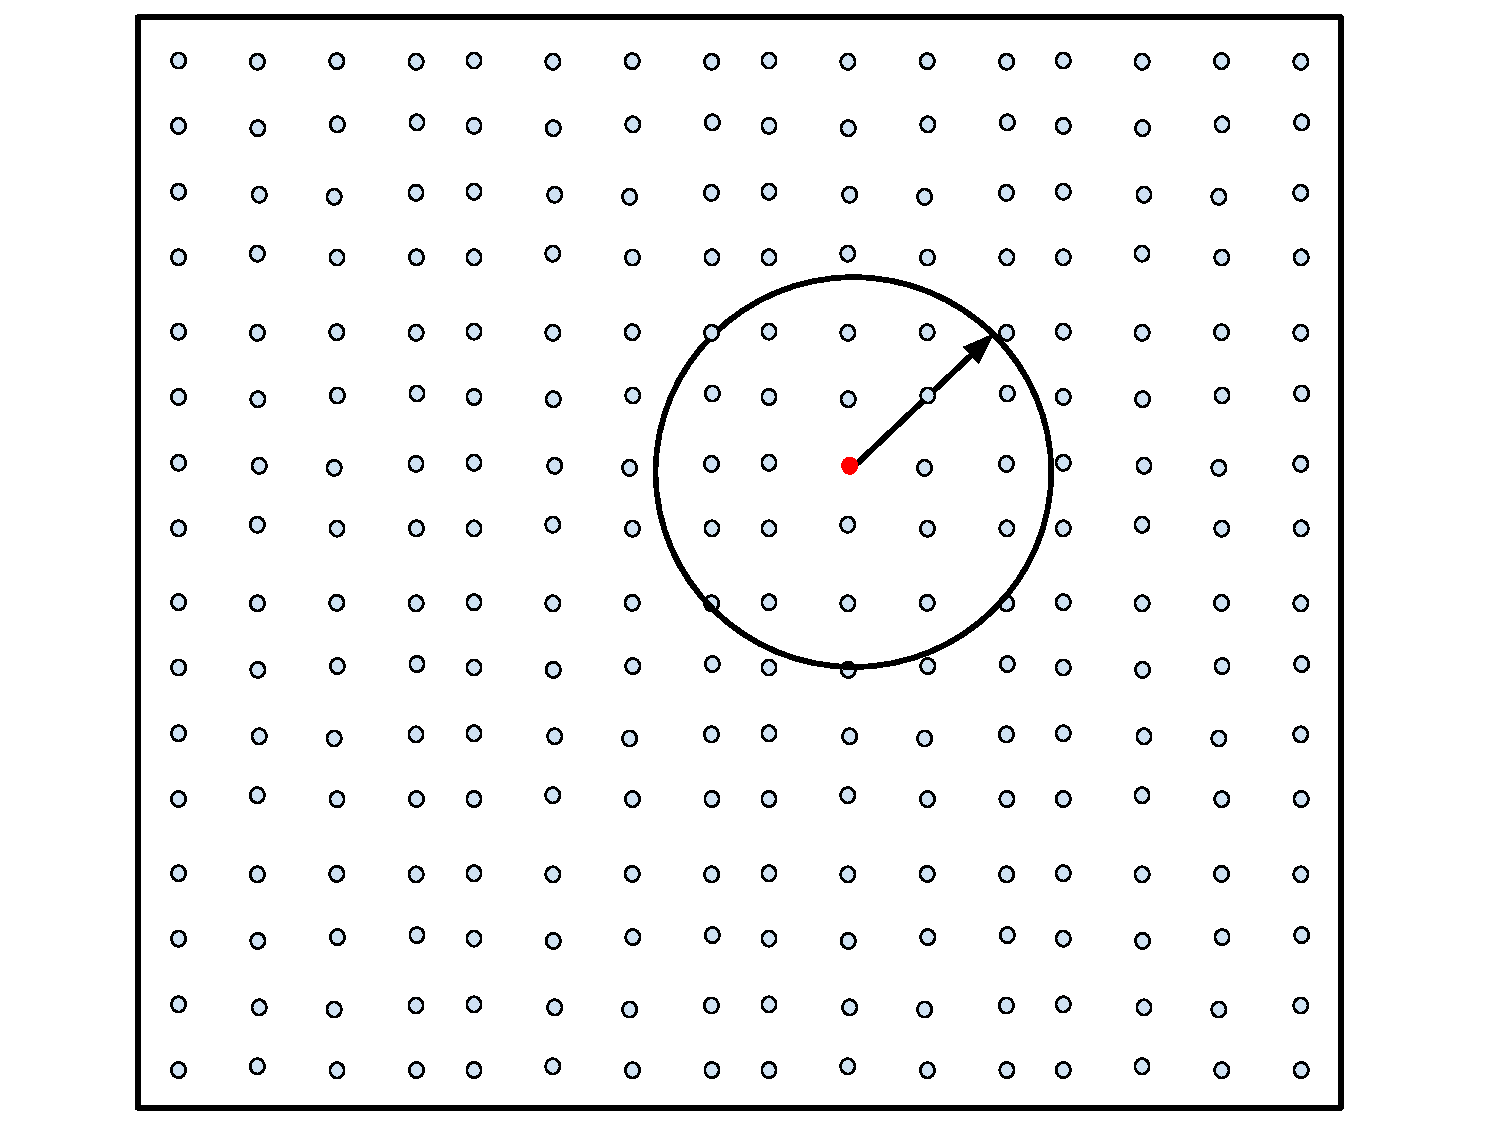
\includegraphics[width=0.415\textwidth]{Neighor-searching-noBG}
\hfill
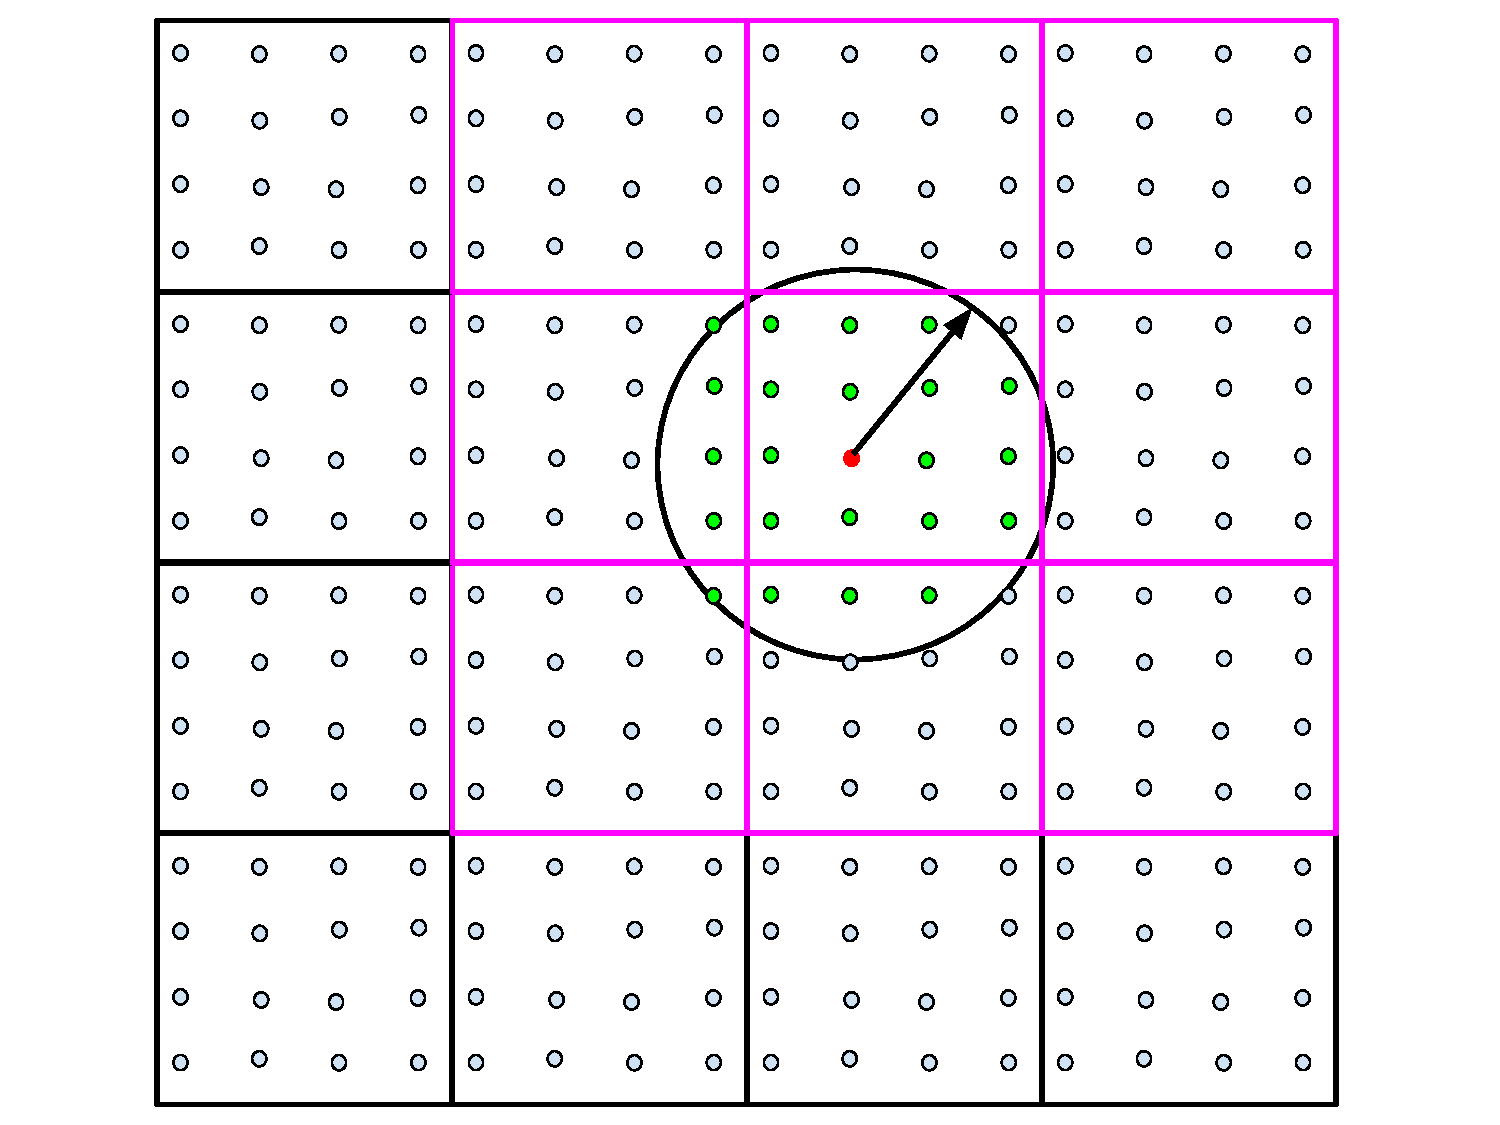
\includegraphics[width=0.415\textwidth]{Neighbor-Search}
\end{figure}
\end{frame}

\begin{frame}{SFC-based Index $\&$ Domain Decomposition}
SFC based key is defined as: $k = h_n (\textbf{x})$, Where $h_n (\textbf{x}): [0,1]^n \rightarrow [0,1]$
\begin{figure}
\flushleft
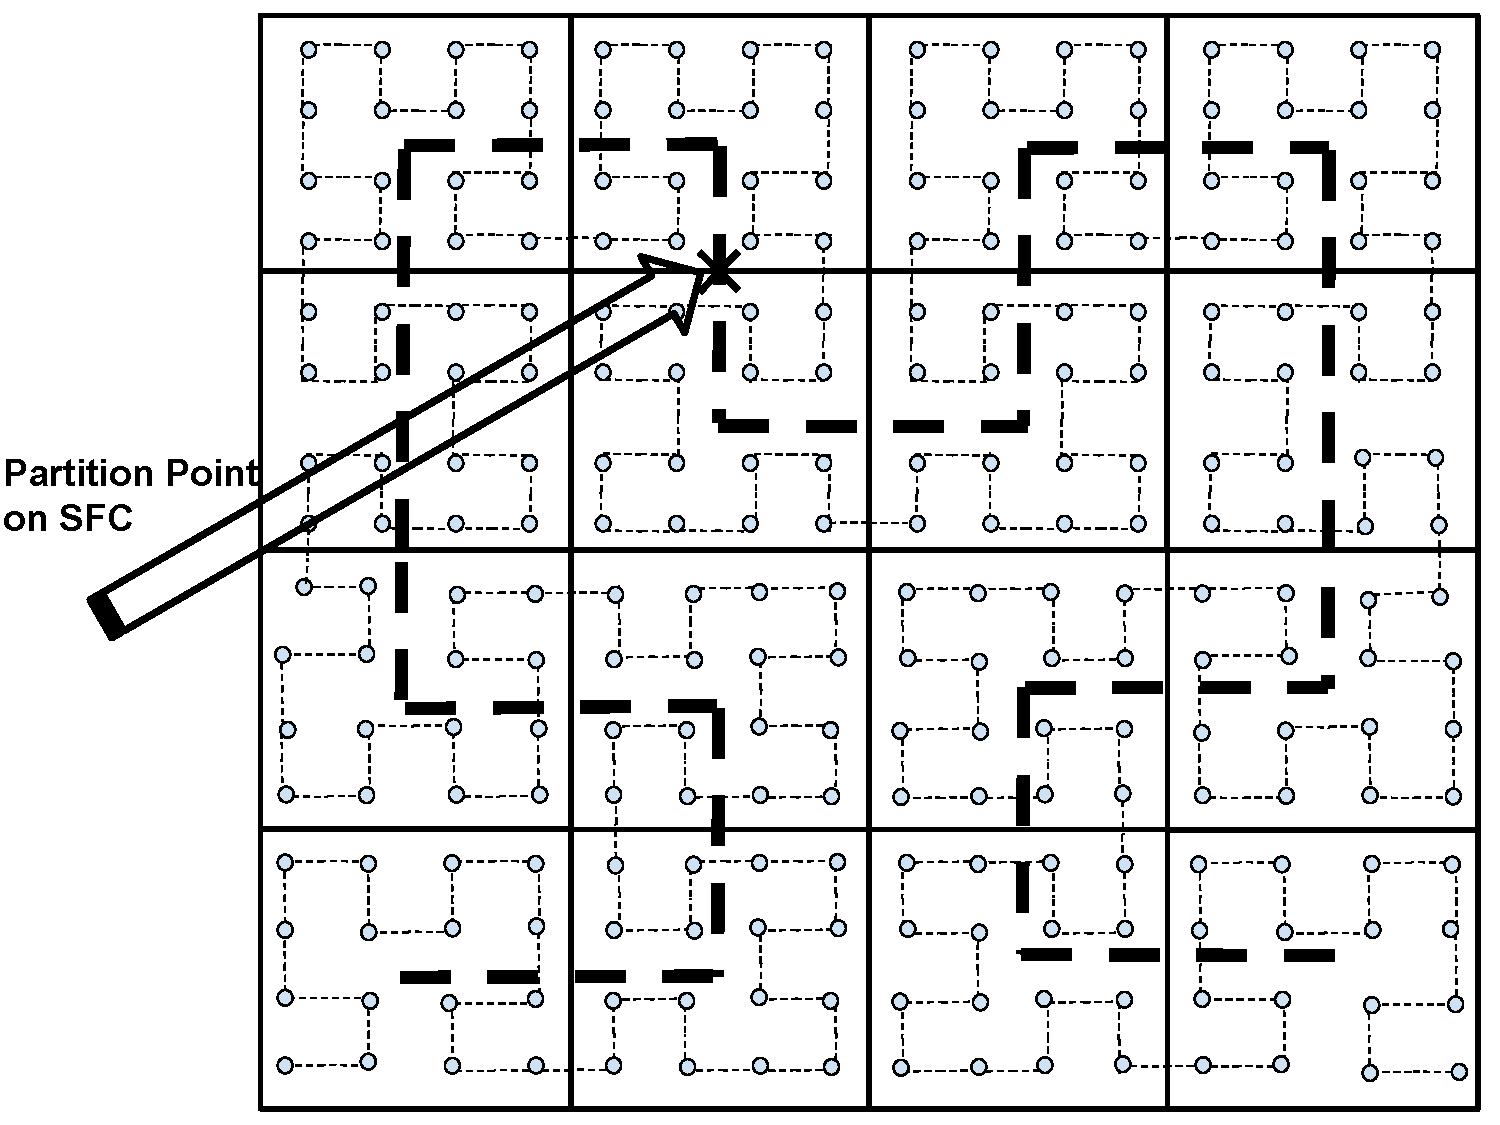
\includegraphics[width=0.385\textwidth]{../SFC_particles_buckets}
\hfill
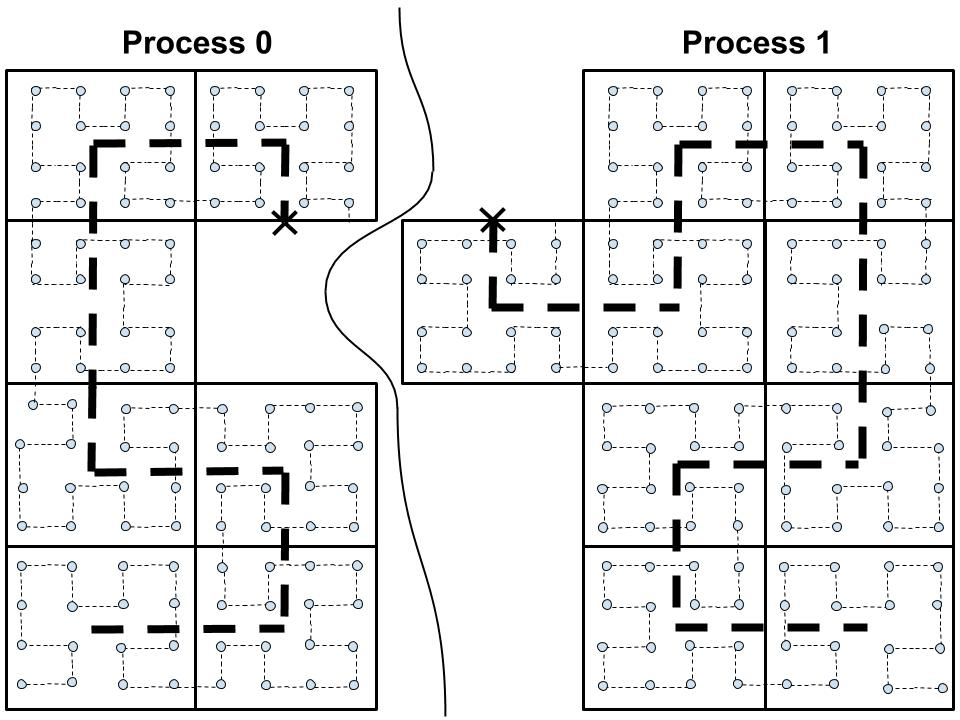
\includegraphics[width=0.415\textwidth]{../SFC_particles_buckets_partition}
\end{figure}
\begin{block}{Features of SFC-based Index}
  \begin{itemize}
  \item {
    Guaranteed uniqueness of the indexing.
  }
  \item {
    Generating of indices are fast and
independent
  }
  \item {
    Conserve spatial locality in ordering $\rightarrow$ promotes memory locality / {\bf cache reuse}
  }
  \item {
    Global address space and ordering for use in  domain decomposition
  }
  \end{itemize}
\end{block}
\end{frame}

\begin{frame}{Eruption BC $\&$ Time-dependent SFC}
\begin{figure}
\flushleft
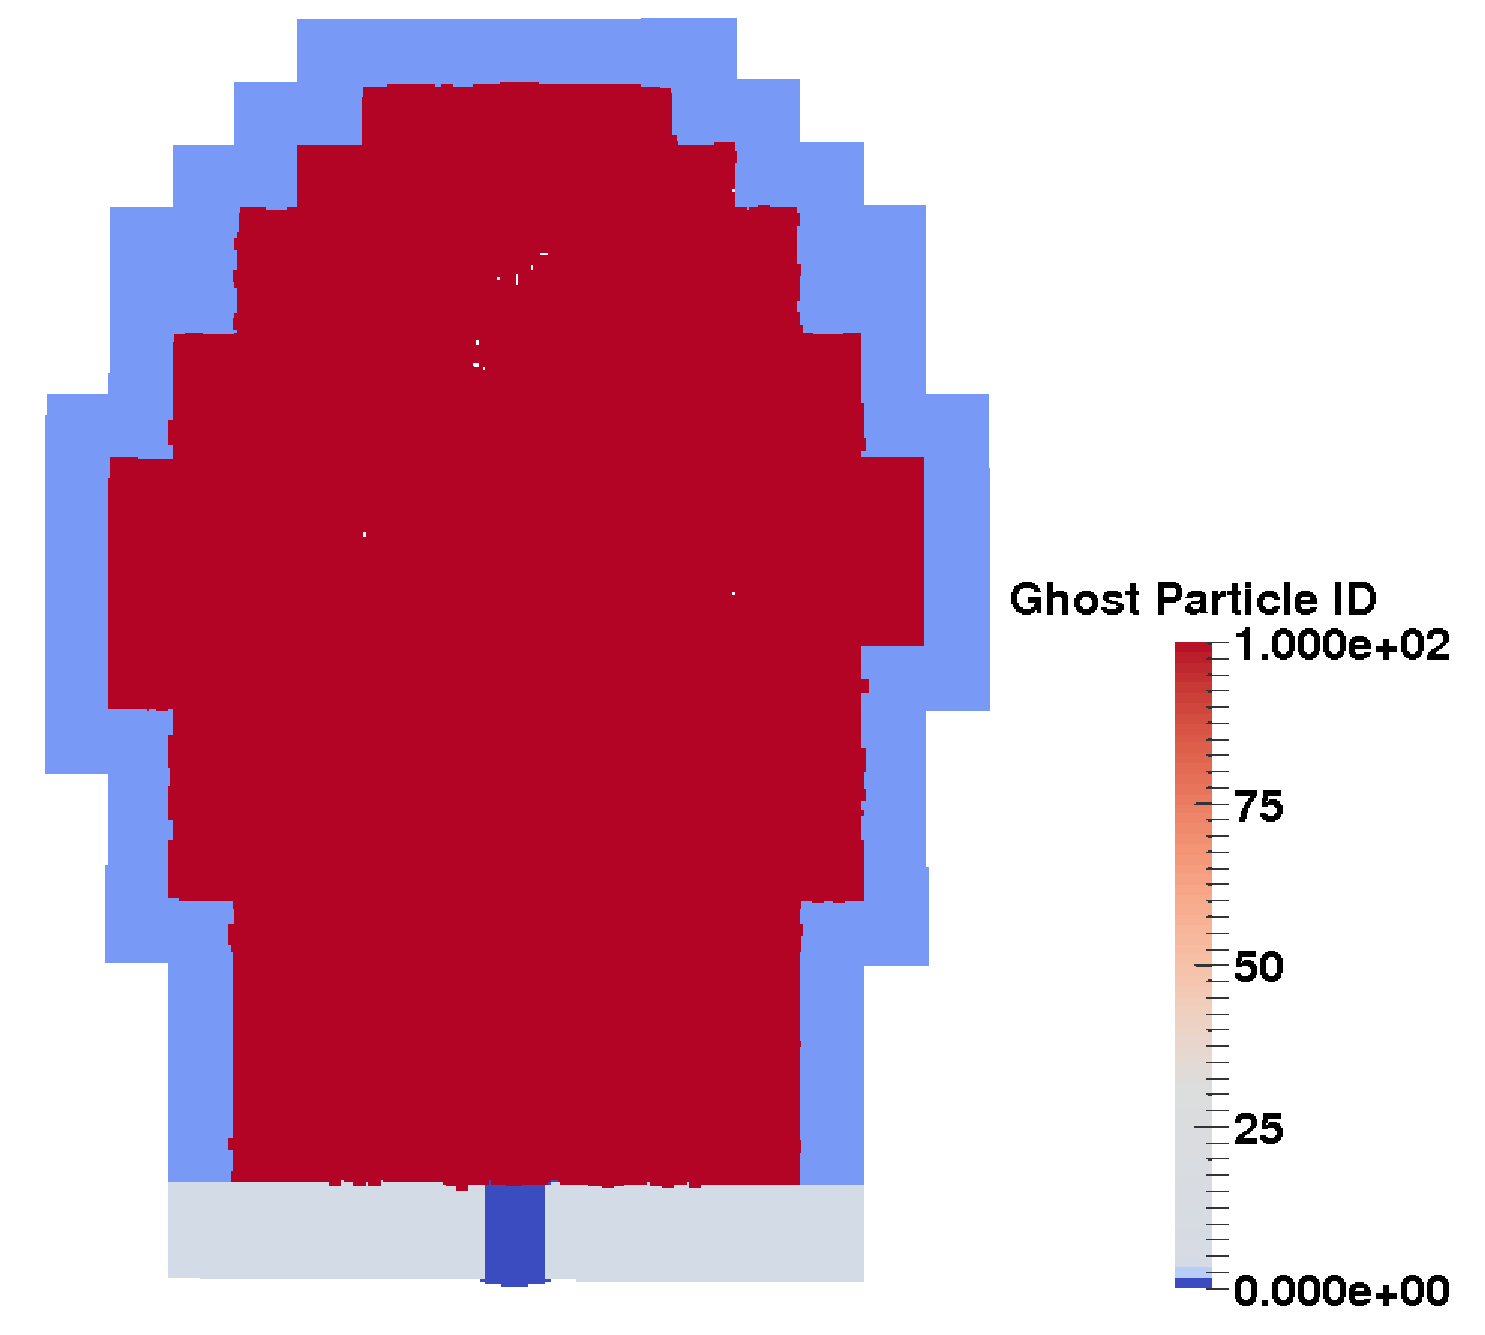
\includegraphics[width=0.435\textwidth]{../Boundary-condition-eps-converted-to}
\hfill
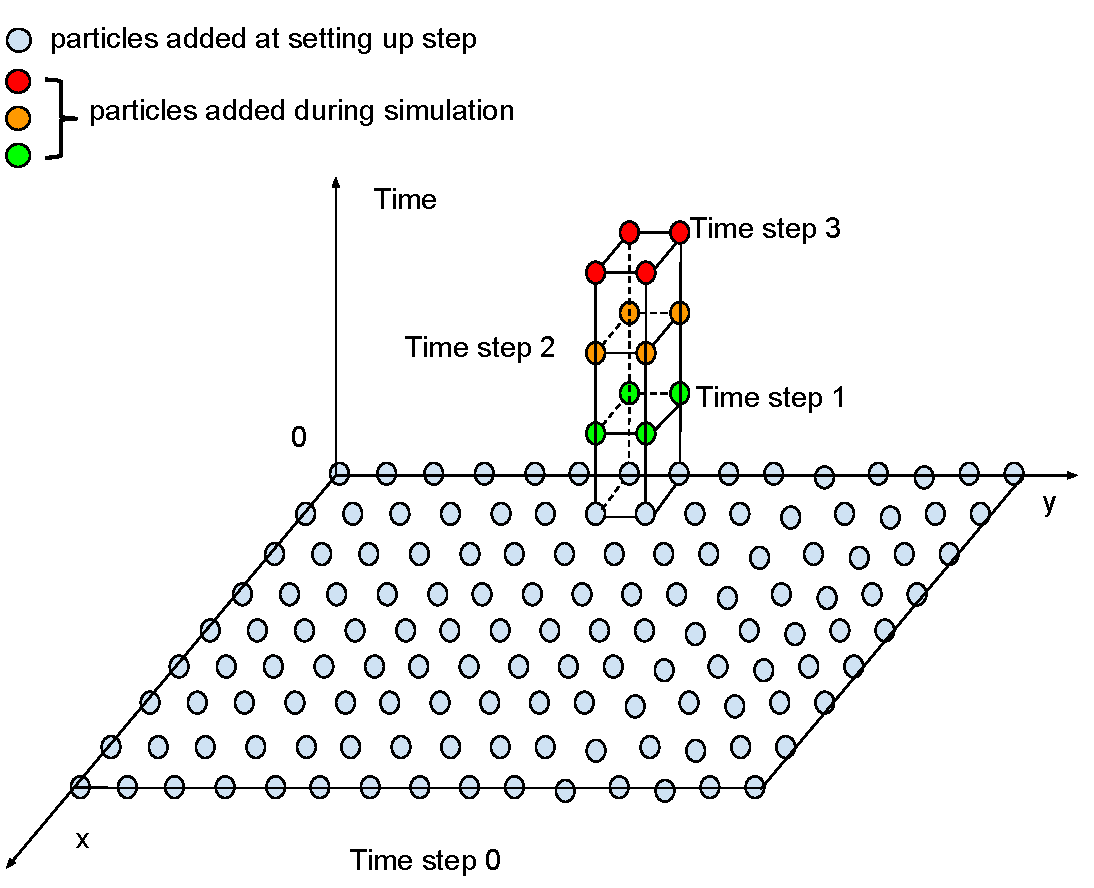
\includegraphics[width=0.445\textwidth]{Particle_adding}
\end{figure}
\begin{block}{Time-dependent SFC}
\begin{equation}
h_n: [0,1]^n \times \textbf{T} \rightarrow [0,1] \times \textbf{N}
\end{equation}
Where $\textbf{T} \subset [0,\infty)$ is the time dimension, and $\textbf{N}=\lbrace 0, 1, 2, 3...\rbrace$. \\
Then the time-dependent key can be expressed as: $(k,n)$
\end{block}
\end{frame}

\begin{frame}{Hash Table with External Linked List}
\begin{figure}
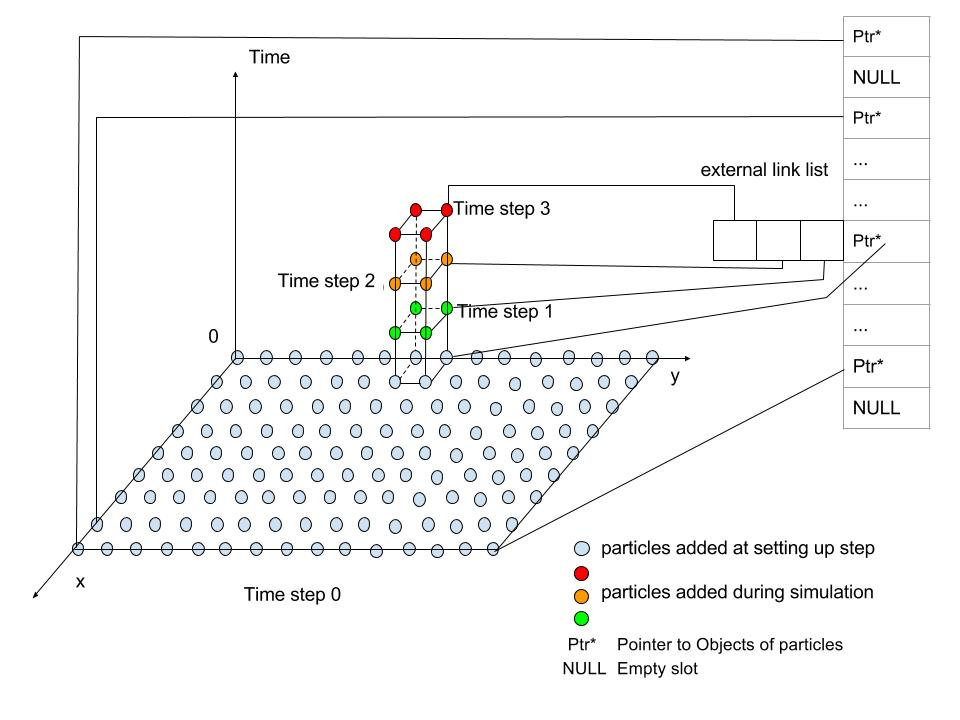
\includegraphics[width=0.55\textwidth]{../Particle_adding_with_link}
\end{figure}
\begin{block}{Hash Function}
\begin{equation}
Index= \frac{Key - Min\,Key}{Max\,Key - Min\,Key} 
\times Hash\,Table\,Size 
\label{eq:hash_function}
\end{equation}
To avoid a non-uniform sparse hash table, only plug the first number, $k$, of the key, into Eq. (\ref{eq:hash_function}). All particles with the same birth location will hash to the same index and be handled by external linked lists.
\end{block}
\end{frame}

\begin{frame}{Dynamic Load Balance (Weighted particles)}
The domain is decomposed by cutting SFC of buckets into pieces of equal work load. The work load of each bucket is calculated by summing up weights of all particles contained by that bucket. The work load associated to each particle is calibrated based on profilling data.
\begin{table}
\resizebox{0.9\textwidth}{!}{  
	  \begin{tabular}{lrrrrrr}
	    \hline
	    Step & Cost ($ms$) & Real & wall & eruption & pressure\\
	    \hline
	    neighbor search & 0.41 & Yes & No & No & No \\
	    update momentum and energy & 0.70 & Yes & No & No & No\\
	    update density & 0.42 & Yes & No & No & No \\
	    update position & 0.01 & Yes & No & Yes &  No\\
	    velocity filtering& 0.43 & Yes & No & No & No\\
	    apply wall boundary condition     & 0.75 & No & Yes & No & No\\
	    summation ($ms$) & - & 1.97 & 0.75 & 0.01 & 0.00\\
	    \hline
	  \end{tabular}}
      \label{tab:Computational_cost_steps}
\end{table}
Compared with uniform particle weight, calibrated particle weights is computationally more efficient.
\begin{table}
\resizebox{0.7 \textwidth}{!}{  
	  \begin{tabular}{lrrrr}
	    \hline
	    Physical time & 10 s & 20s & 30 s & 40 s \\
	    \hline
	    Same weight & 1141.7 & 4119.4 & 10371.0 & 12453.7\\
	    Calibrated weights & 1108.2 & 4057.0 & 10281.5 & 12166.3 \\
	    \hline
	  \end{tabular}}
      \label{tab:effect-of-weighted-particle}
\end{table}

\end{frame}

\begin{frame}{Dynamic Load Balance (Load check interval)}
The movement of particles and expansion of computational domain can lead to large load imbalance. 
\begin{figure}
\flushleft
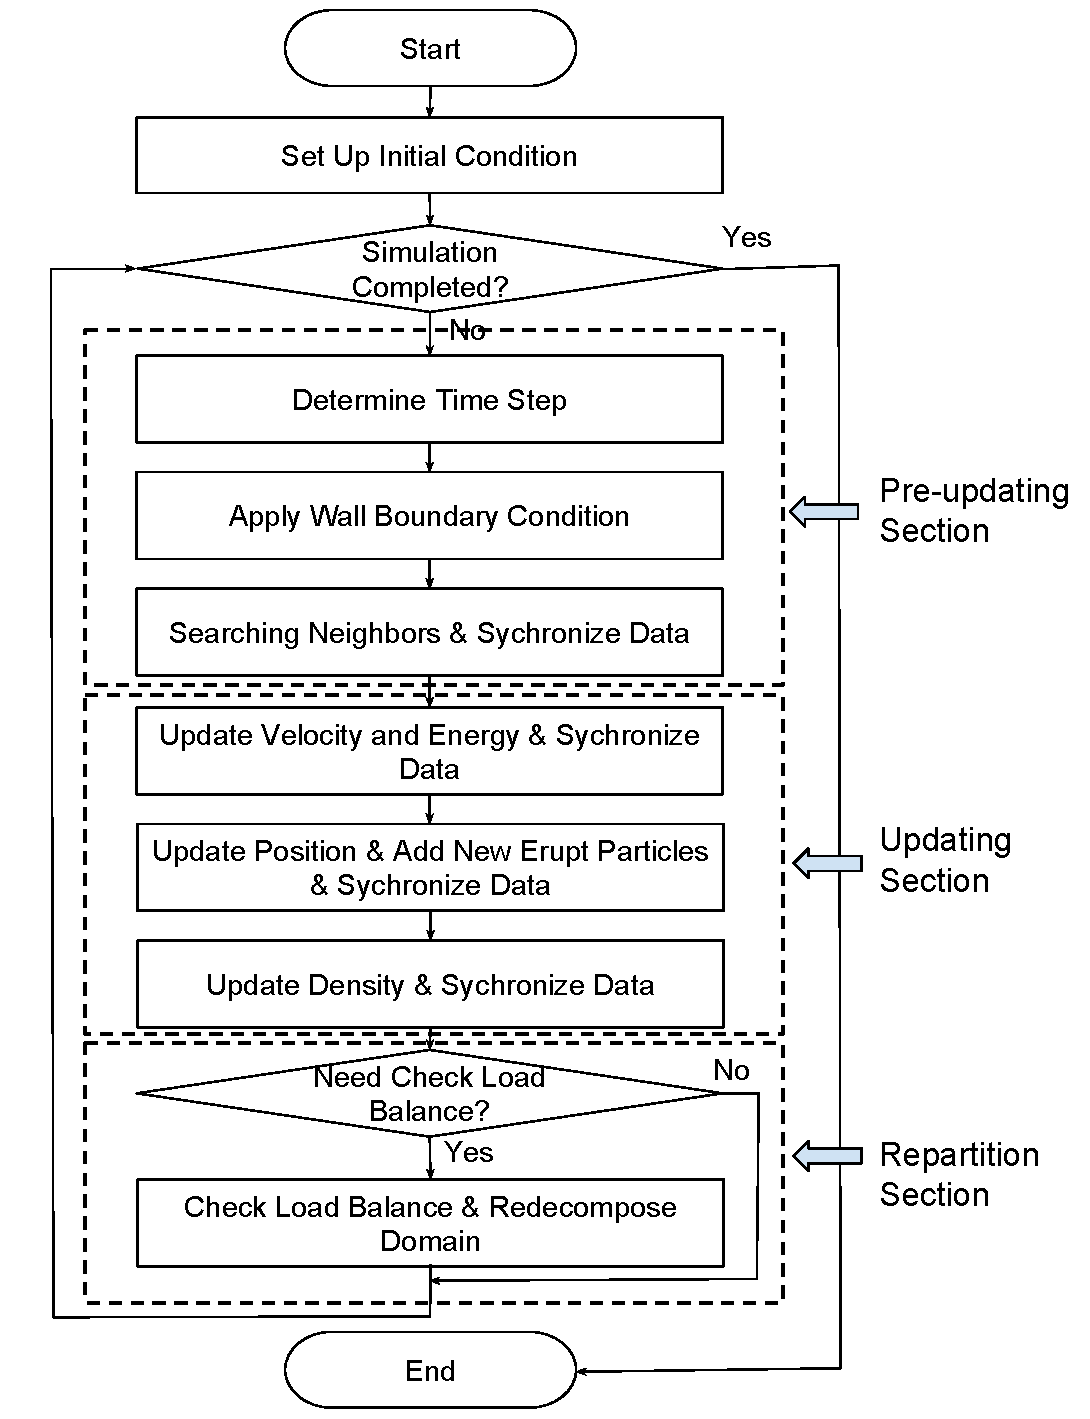
\includegraphics[width=0.435\textwidth]{../Work_flow}
\hfill
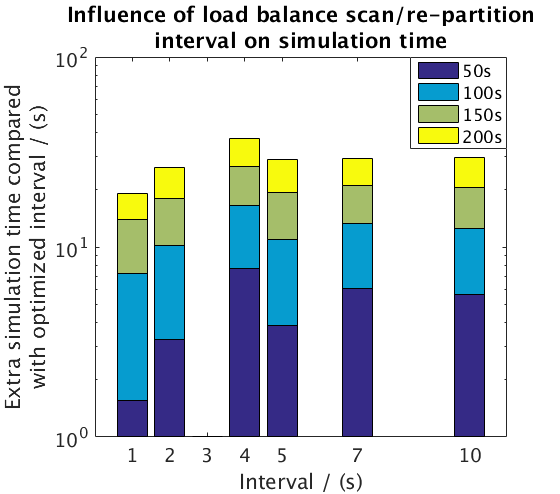
\includegraphics[width=0.445\textwidth]{../int_bar}
\end{figure}
\end{frame}

%---------------------------------------------------------
\section{Dynamic Halo Domain}
\begin{frame}{Dynamic Halo Domain}
A lot of CPU time will be spent
on computing associated with these stationary particles. The computational cost will be greatly reduced if the computational domain changes adaptively during simulation. 
\begin{block}{Our strategy}
  \begin{itemize}
  \item {
    An involvement flag to distinguish different states of involvement
  }
  \item {
    A scan function to monitor the outermost layer of the domain
  }
  \item {
    Shift pressure ghost particles into real particles when necessary
  }
  \end{itemize}
\end{block}
%
\begin{figure}
\flushleft
\includegraphics[width=0.33\textwidth]{t=66_msfrc}
\hfill
\includegraphics[width=0.33\textwidth]{t=66_bctp}
\hfill
\includegraphics[width=0.33\textwidth]{t=66_involved}
\end{figure}
\end{frame}

\begin{frame}{Dynamic Halo Domain}
%
\begin{figure}[!tbp]
%
\begin{minipage}[b]{0.39\textwidth}
\begin{figure}
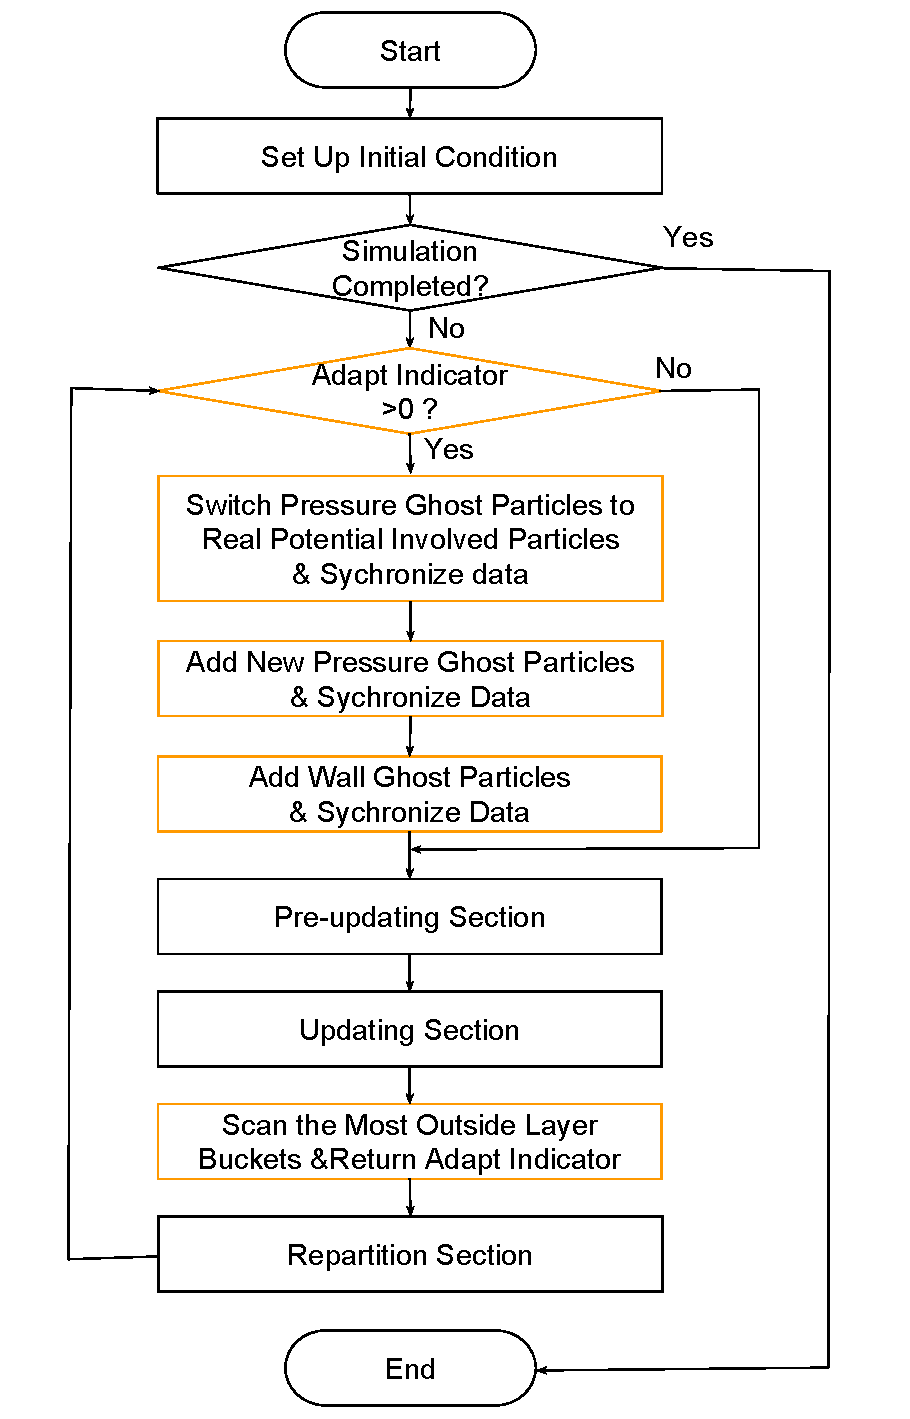
\includegraphics[width=\textwidth]{../Work_flow_adjust}
\end{figure}
\end{minipage}
\hfill
\begin{minipage}[b]{0.60\textwidth}
\begin{scriptsize}
\linespread{1.0}{
SWCH: switch pressure ghost particles to real. ADPP: add new pressure ghost particles. ADWP: add wall ghost particles. SCN: scann the outmost layer of the domain}
\end{scriptsize}
\center
\resizebox{0.70 \textwidth}{!}{
    \begin{tabular}{lrr}
    \hline
    Functions & Total time (s) & Called times\\
    	\hline
    UPME & 2954.8 & 201 \\
    UPP & 38.55 &  201 \\
    ADPP & 21.51 & 3 \\
    ADWP  & 8.88 & 3 \\
    SWCH & 0.08 &  2 \\
    SCN  & 7.72 & 201 \\
    \hline
  \end{tabular}}
\begin{figure}
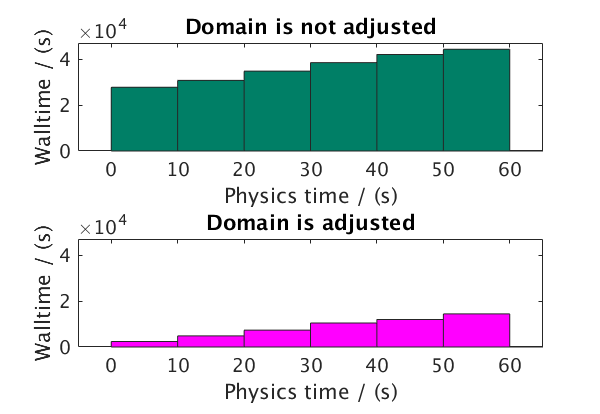
\includegraphics[width=0.70\textwidth]  {../adj_vs_no}
\end{figure}
\end{minipage}
%
\end{figure}
\end{frame}
%----------------------------------------------------------------------------
\section{Numerical Test}
\begin{frame}{Scalability}
\begin{figure}
\flushleft
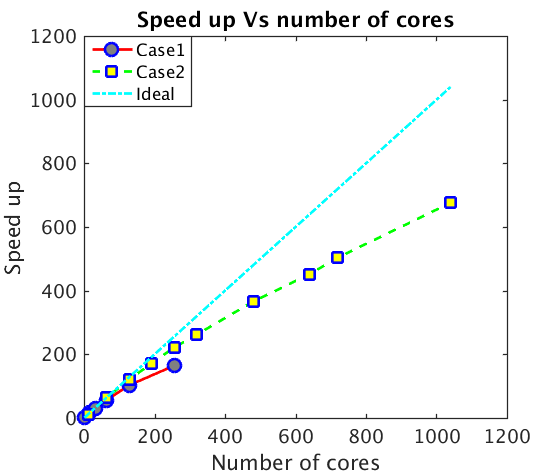
\includegraphics[width=0.31\textwidth]{../strong_scale}
\hfill
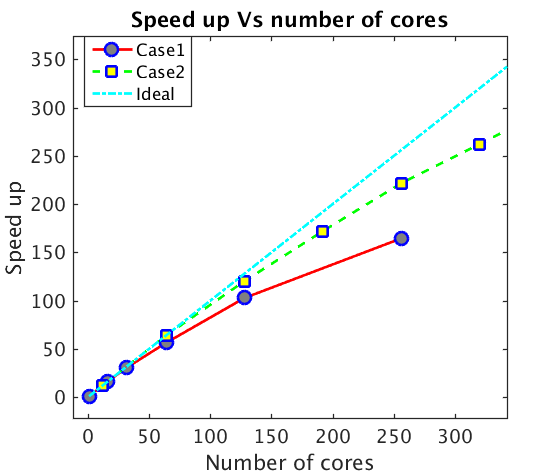
\includegraphics[width=0.31\textwidth]{../strong_scale_zoom}
\hfill
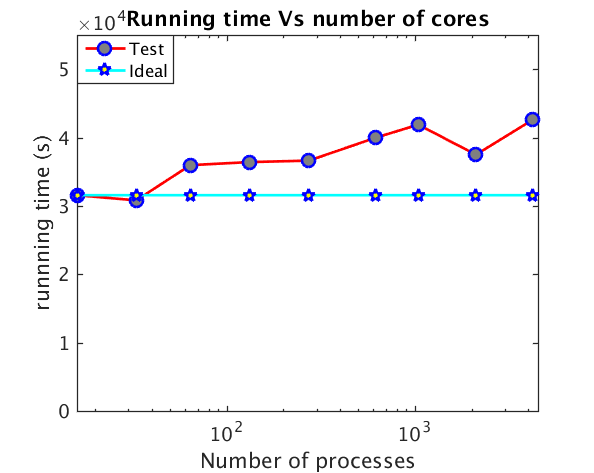
\includegraphics[width=0.31\textwidth]{../weak_scale}
\caption{The left figure shows strong scalability tests result. middle figure is the zoomed view of first one. It is obviously shown that strong scalability is better when the problem size is larger. The right figure is weak scalability test results}
\label{fig:2cases_efficiency}
\end{figure}
%
\end{frame}

\begin{frame}{A Typical Simulation Results}
%
\begin{minipage}{.32\linewidth}
\includemedia[
  label=vidA,
  width=0.99\linewidth,
  height=1.3\linewidth,
  activate=onclick,
  deactivate=onclick,
  addresource=mssfrc_sml400.mp4,
  flashvars={source=mssfrc_sml400.mp4 &loop=true}
  ]{}{VPlayer.swf}
\end{minipage}
\hfill
\begin{minipage}{.32\linewidth} 
  \includemedia[
  label=vidB,
  width=0.99\linewidth,
  height=1.3\linewidth,
  activate=onclick,
  deactivate=onclick,
  addresource=cut_view_mssfrc_sml400.mp4,
  flashvars={source=cut_view_mssfrc_sml400.mp4 &loop=true}]
  {}{VPlayer.swf}
\end{minipage}
\hfill  
\begin{minipage}{.32\linewidth} 
  \includemedia[
  label=vidC,
  width=0.99\linewidth,
  height=1.3\linewidth,
  activate=onclick,
  deactivate=onclick,
  addresource=cut_view_Involved_sml400.mp4,
  flashvars={source=cut_view_Involved_sml400.mp4 &loop=true}]
  {}{VPlayer.swf}
\end{minipage}
%  
  \mediabutton[
  mediacommand=vidA:playPause,
  mediacommand=vidB:playPause,
  mediacommand=vidC:playPause,
]{\fbox{Play/Pause}}
%
\end{frame}

%\begin{frame}{Blocks}
%\begin{block}{Block Title}
%You can also highlight sections of your presentation in a block, with it's own title
%\end{block}
%\begin{theorem}
%There are separate environments for theorems, examples, definitions and proofs.
%\end{theorem}
%\begin{example}
%Here is an example of an example block.
%\end{example}
%\end{frame}
% Placing a * after \section means it will not show in the
% outline or table of contents.
%----------------------------------------------------------------------------
\section*{Summary}

\begin{frame}{Requirements of the application}
\begin{figure}[!t]
\centering
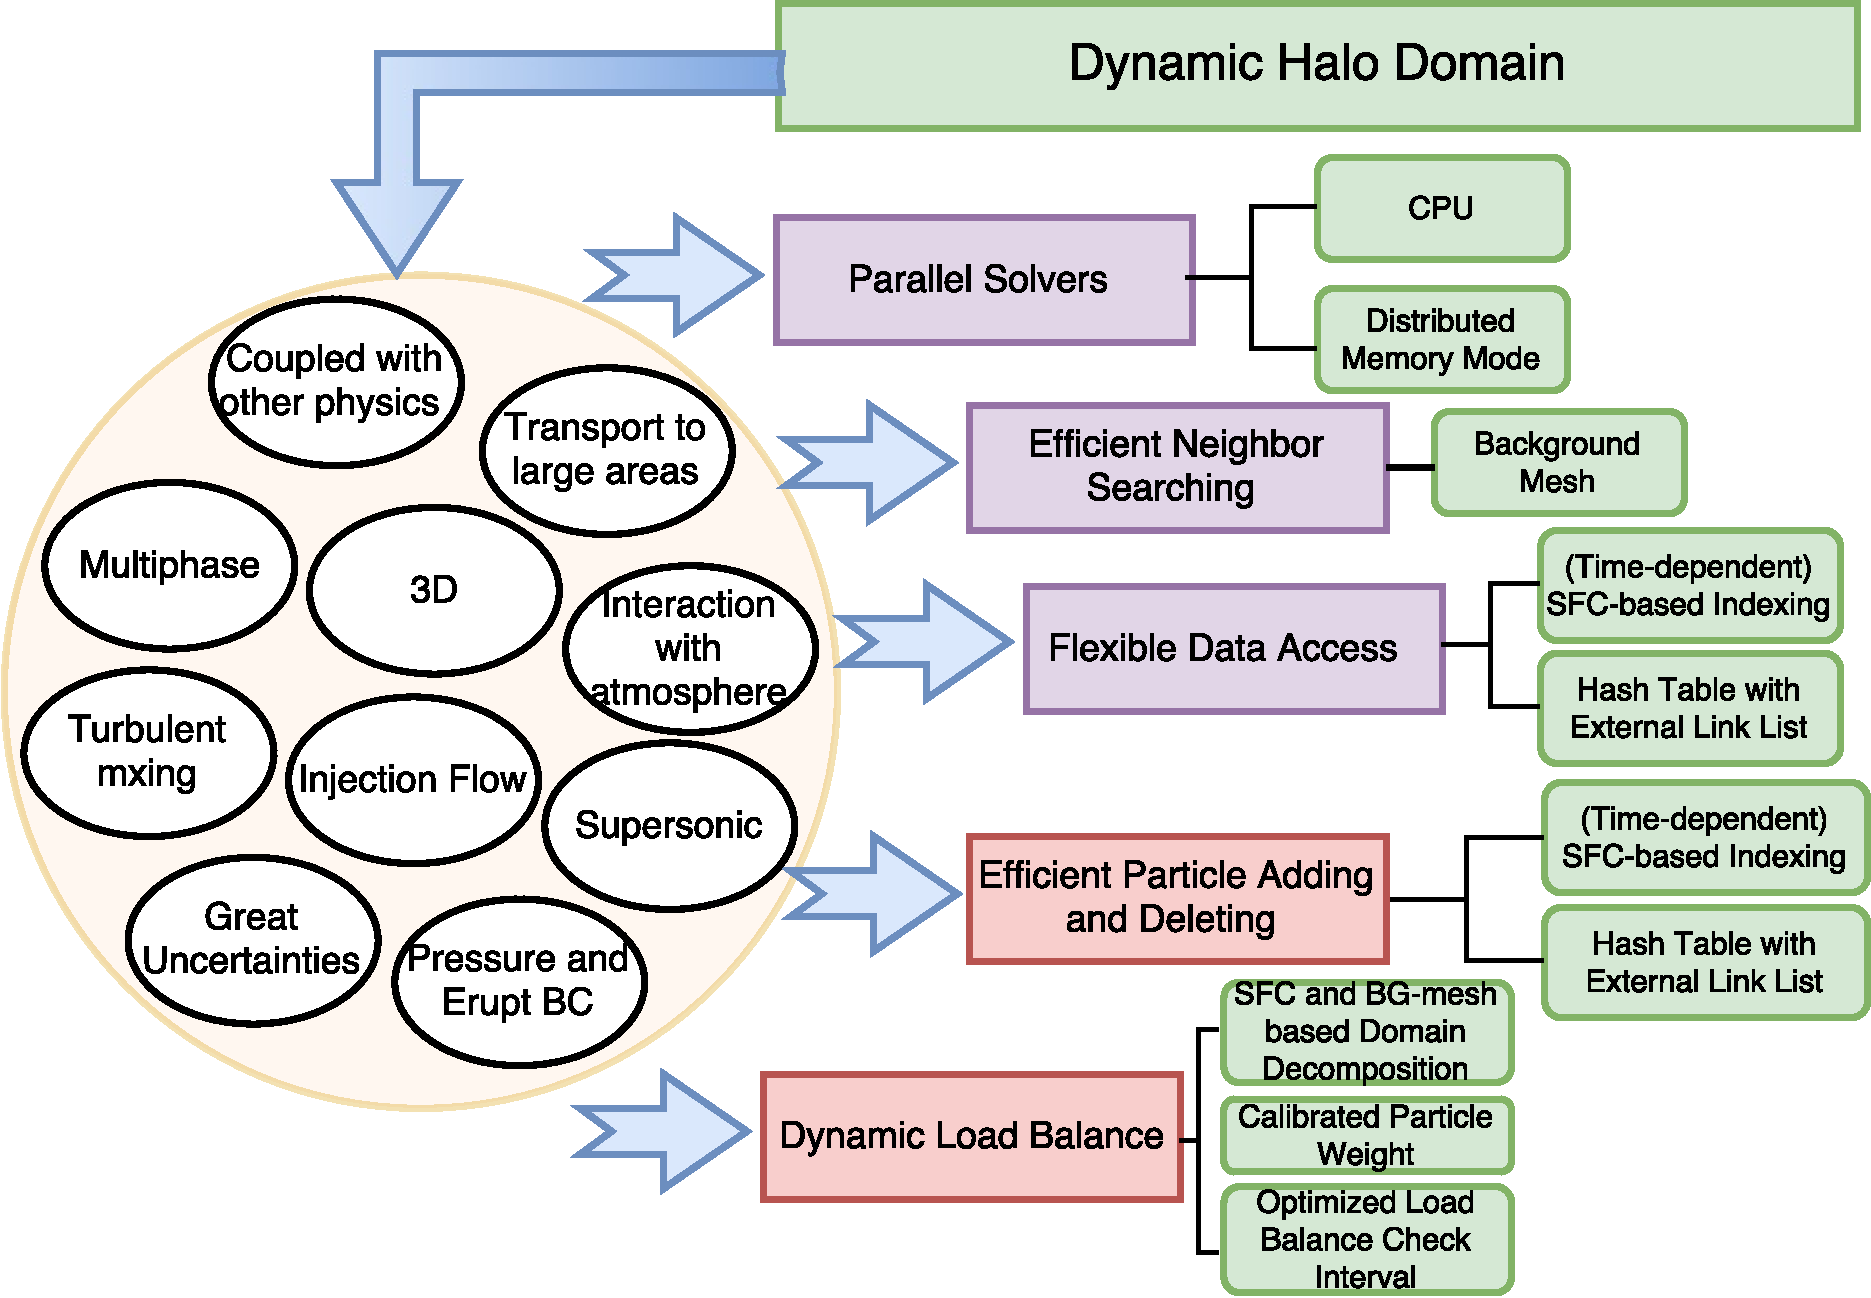
\includegraphics[scale=0.35]{Requirement_all}
%\caption{Scope of the problem}
\label{fig:Requirements}
\end{figure}
\end{frame}

\begin{frame}{Summary}
  \begin{itemize}
  \item
    We developed data management strategies for a MPI-parallel implementation of the SPH
method to simulate volcanic plumes. Acceptable scalability was achieved.
  \item
    The flexibility of our data access methodology enables implementation of  mesh-free methods for
solving more complicated problems and using more advanced techniques, such as dynamic particle splitting techniques.
  \item
    The data structure, particle and bucket
indexing strategies, domain decomposition, dynamic load balancing method and domain ad-
justing strategies in this paper can be adopted by other mesh-free methods (not just SPH).
  \end{itemize}
  
  \begin{itemize}
  \item
    Current/Future
    \begin{itemize}
    \item
      Better dynamic load balancing strategy.
    \item
      Adaptive background grid and better domain decomposition algorithm.
    \end{itemize}
  \end{itemize}
\end{frame}

\begin{frame}{Summary}
\center
\Huge{
Thank you! \\
Questions are welcome.
}
\end{frame}

%% All of the following is optional and typically not needed. 
%\appendix
%\section<presentation>*{\appendixname}
%\subsection<presentation>*{For Further Reading}
%
%\begin{frame}[allowframebreaks]
%  \frametitle<presentation>{For Further Reading}
%    
%  \begin{thebibliography}{10}
%    
%  \beamertemplatebookbibitems
%  % Start with overview books.
%
%  \bibitem{Author1990}
%    A.~Author.
%    \newblock {\em Handbook of Everything}.
%    \newblock Some Press, 1990.
% 
%    
%  \beamertemplatearticlebibitems
%  % Followed by interesting articles. Keep the list short. 
%
%  \bibitem{Someone2000}
%    S.~Someone.
%    \newblock On this and that.
%    \newblock {\em Journal of This and That}, 2(1):50--100,
%    2000.
%  \end{thebibliography}
%\end{frame}

\end{document}


